\documentclass{article}
\usepackage{amsmath}
\usepackage{mathptmx}
\usepackage{tikz}
\usepackage{pgfplots}
\usepgfplotslibrary{colormaps}
\usepgfplotslibrary{patchplots}
\usepgfplotslibrary{polar}
\usepgfplotslibrary{fillbetween}
\usepackage{tkz-fct}
\usetikzlibrary{angles, quotes}
\usetikzlibrary{arrows.meta, arrows}
\usetikzlibrary{external}
\tikzexternalize[prefix={external/}]

\definecolor{myblue}{rgb}{0.067,0.529,0.871}
\definecolor{mypurple}{rgb}{0.859,0.071,0.525}
\definecolor{myred}{rgb}{1.0, 0.13, 0.32}
\definecolor{mygreen}{rgb}{0.01, 0.75, 0.24}
\definecolor{myblack}{gray}{0.5}
\definecolor{mygray}{gray}{0.7}

\pgfplotsset{
    compat=newest,
    colormap={bluemap}{color=(myblue) color=(myblue!25) color=(myblue!50)},
    colormap={redmap}{color=(myred) color=(myred!25) color=(myred!50)}
}

\tikzset{
    export as png/.style={
        external/system call/.add={}{
            && convert -density #1 -transparent white "\image.pdf" "\image.png"
        },
    },
    export as png/.default={200},
}

\DeclareSymbolFont{symbolsb}{OMS}{cmsy}{m}{n}
\SetSymbolFont{symbolsb}{bold}{OMS}{cmsy}{b}{n}
\DeclareSymbolFontAlphabet{\mathcal}{symbolsb}
\definecolor{myblue}{rgb}{0.067,0.529,0.871}
\definecolor{mypurple}{rgb}{0.859,0.071,0.525}
\definecolor{myred}{rgb}{1.0, 0.13, 0.32}
\definecolor{mygreen}{rgb}{0.01, 0.75, 0.24}
\definecolor{myblack}{gray}{0.5}
\definecolor{mygray}{gray}{0.7}

\def\req{\protect\rotatebox{90}{$\scriptstyle=$}}

\begin{document}

\tikzset{export as png}

\tikzsetnextfilename{esfera}
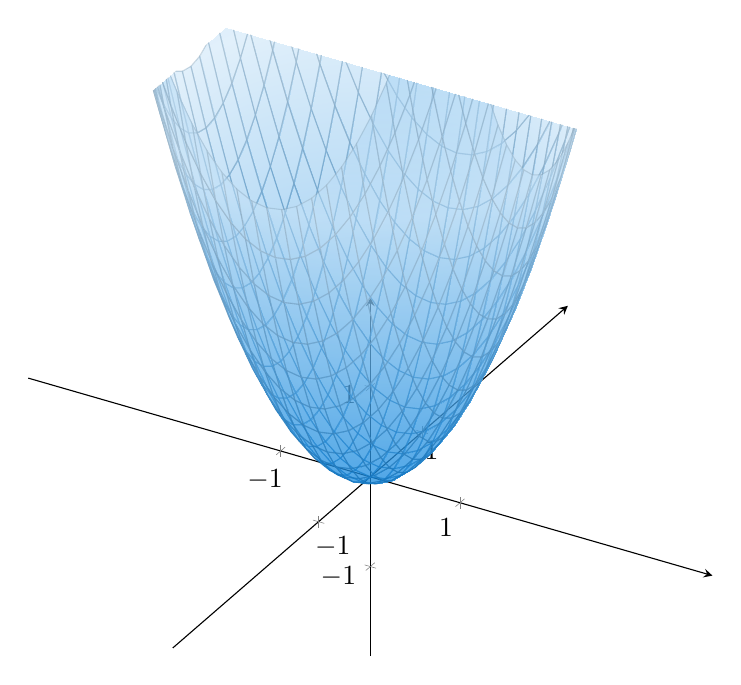
\begin{tikzpicture}
    \begin{axis}
    [   axis equal,
        axis lines=center,
        xmin = -2, xmax = 2,
        ymin = -2, ymax = 2, 
        zmin = -2, zmax = 2,
        xtick = {-1,0,1},
        ytick = {-1,0,1},
        ztick = {-1,0,1},
        %axis on top,
        view={30}{30},
        z buffer=sort,
        colormap name = bluemap,
        scale = 2
    ]
        \addplot3
        [   domain = -2:2,
            y domain = -2:2,
            surf,
            shader=faceted interp,
            opacity=0.5,
        ] (x, y, x^2+y^2);
    \end{axis}
\end{tikzpicture}
\end{document}


